\documentclass[slovene,11pt,a4paper]{article}

\usepackage[margin=1.5cm,bottom=3cm,foot=1.5cm]{geometry}
\usepackage{amsmath}
\usepackage{booktabs}
\usepackage{float}
\usepackage{graphicx}
\usepackage{changepage}
\usepackage{subcaption}
\usepackage{multirow}
\usepackage{blindtext}
\usepackage{hyperref}
\usepackage[version=4]{mhchem}
\usepackage[slovene]{babel}


\pagenumbering{gobble}

\begin{document}

\title{6. naloga \\ Gručenje v hadronske curke}
\author{Tadej Lozej 28242023}
\maketitle

\begin{center}
Praktikum strojnega učenja v fiziki \\
\bigskip
Predavatelja: red. prof. dr. Borut Paul Kerševan, doc. dr. Simon Čopar \\
Asistent: Blaž Bortolato
\end{center}

\newpage

\tableofcontents

\newpage

\pagenumbering{arabic}

\section{Uvod}

Pri trkih visokoenergijskih delcev se pogosto pojavijo hadronski curki, ki jih zaznajo s posebnimi detektorji. Hadroni so sestavljeni iz kvarkov, ki jih veže močna interakcija. Prostih kvarkob ni mogoče zaznati, saj se hitro vežejo v hadrone. Vprašanje o tem kako se med seboj vežejo želimo povezati z eksperimentalnimi meritvami, ki jih lahko opravimo s pomočjo detektorjev. V tem poročilu bomo uporabili strojno učenje za analizo podatkov iz trkov delcev in preučili, kako se hadronski curki oblikujejo.

V primeru, ko v nekem procesu pričakujemo dva kvarka, se v meritvi pričakuje dva hadronska curka. V praksi je število curkov večje, saj lahko začetna stanja trkov sevajo gluone. Cilj naloge je ločiti hadronske curke med seboj ter izluščiti le dva z najvišjo energijo, saj sta ta dva povezana z osnovnim procesom.

Podatki so v obliki seznama delcev, ki jih zazna detektor. Vsak delec ima svojo tranzverzalno gibalno količino $p_T$, pseudorapidnost $\eta$ in azimutalni kot $\phi$. Na podlagi teh podatkov bomo uporabili algoritme gručenja, da bomo izluščili hadronske curke.

Kot algoritme gručenja bomo uporabili K-means ter hierarhično gručenje. Naloga prvega je, da razdeli množico s številom točk $N$ v $K$ skupin, pri čemer je $K$ vnaprej določeno število. Algoritem deluje tako, da izbere $K$ naključnih točk kot začetne centre skupin. Nato vsako točko dodeli najbližjemu centru in na koncu izračuna nove centre skupin kot povprečje točk v posamezni skupini. Postopek se ponavlja, dokler se centri ne stabilizirajo.

Hierarhično gručenje deluje drugače. Seznam delcev, ki jih izmerimo imenujmo seznam protocurkov. Seznam, ki ga dobimo po gručenju, imenujmo seznam pravih curkov. Na začetku je ta seznam prazen in se polni med potekom algoritma. Algoritem ima prost parameter $R$, ki je sorazmeren z radijem pravih curkov. Za vsak protocurek izračunamo količino $d_i = p_{T,i}^{2p}$ ter za vsak par protocurkov izračunamo količino

\begin{equation}
    d_{ij} = \min(p_{T,i}^{2p}, p_{T,j}^{2p}) \frac{\Delta \eta_{ij}^2 + \Delta \phi_{ij}^2}{R^2},
\end{equation}
kjer sta $\Delta \eta_{ij}$ in $\Delta \phi_{ij}$ razlika pseudorapidnosti in azimutalnega kota med $i$-tim in $j$-tim protocurkom. Nato izračunamo najmanjšo količino $d_{\min} = \min(d_i, d_{ij})$. Če je $d_{\min} = d_i$, potem protocurek $i$ dodamo v seznam pravih curkov. Če pa je $d_{\min} = d_{ij}$, potem združimo protocurka $i$ in $j$ v enega in ga dodamo v seznam protocurkov. Postopek se ponavlja, dokler seznam protocurkov ni prazen.

Z izbiro parametra $p$ lahko dobimo različne algoritme. Za $p=1$ dobimo $k_t$-algoritem, za $p=0$ Cambridge-Aachen algoritem in za $p=-1$ anti-$k_t$ algoritem.

\section{K-means na dveh Gaussovih porazdelitvah}

Gručenje na dveh Gaussovih porazdelitvah je preprost primer, ki ga lahko rešimo z algoritmom K-means. V tem primeru imamo dve skupini točk, ki sta porazdeljeni po Gaussovi porazdelitvi. Algoritem K-means bo poskušal najti dva centra skupin in razdeliti točke v dve skupini.

Implementirani algoritem sem pognal dvajsetkrat, da sem se izognil lokalnim minimumom. Rezultati so prikazani na sliki \ref{fig:kmeans_gauss}. Na sliki so prikazane točke, ki so porazdeljene po dveh Gaussovih porazdelitvah, ter končni centroidi, ki jih je našel K-means algoritem.


\begin{figure}[h!]
    \centering
    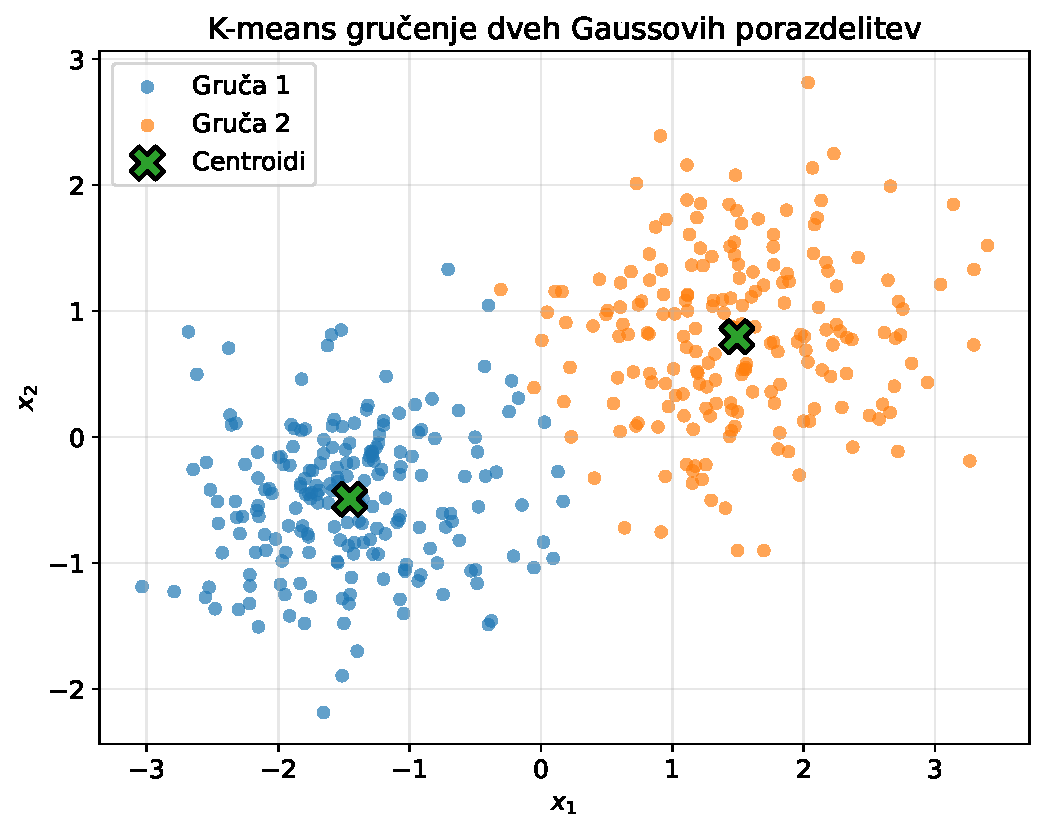
\includegraphics[width=0.75\textwidth]{imgs/kmeans_gauss.pdf}
    \caption{Dve Gaussovi porazdelitvi in končni centroidi K-means algoritma.}
    \label{fig:kmeans_gauss}
\end{figure}


Iz točk porazdelitev lahko določimo povprečji ($\mu_x$ in $\mu_y$) ter standardna odklona dveh porazdelitev ($\sigma_x$ in $\sigma_y$). Tabela \ref{tab:kmeans_gmm_comparison} prikazuje primerjavo rezultatov metode K-means in Gaussian Mixture Model (GMM) iz knjižnice \texttt{skearn}. Rezultati so podobni, kar kaže na to, da je K-means algoritem primeren za ta problem. V tabeli $N$ predstavlja število točk v posamezni gruči.


\begin{table}[h!]
    \centering
    \begin{tabular}{llrrrrr}
        \toprule
        Metoda & Porazdelitev & N & $\mu_x$ & $\mu_y$ & $\sigma_x$ & $\sigma_y$ \\
        \midrule
        K-means & Gauss 1 & 203 & -1.4547 & -0.4926 & 0.6472 & 0.5711 \\
        GMM & Gauss 1 & 194 & -1.4992 & -0.5195 & 0.6126 & 0.5476 \\
        K-means & Gauss 2 & 197 & 1.4924 & 0.7956 & 0.7283 & 0.6703 \\
        GMM & Gauss 2 & 206 & 1.4281 & 0.7746 & 0.7883 & 0.6774 \\
        \bottomrule
    \end{tabular}
    \caption{Primerjava rezultatov metode K-means in Gaussian Mixture Model.}
    \label{tab:kmeans_gmm_comparison}
\end{table}


\section{K means na hadronskih curkih}

V tem poglavju bomo uporabili K-means algoritem za gručenje hadronskih curkov. Podatki so v obliki seznama delcev, ki jih zazna detektor. Vsak delec ima svojo tranzverzalno gibalno količino $p_T$, pseudorapidnost $\eta$ in azimutalni kot $\phi$. Na podlagi teh podatkov bomo uporabili K-means algoritem, da bomo izluščili hadronske curke.

Gručili bomo curke v prvem dogodku, ki je prikazan na sliki \ref{fig:event_display}. Na sliki so prikazani delci, ki jih je zaznal detektor. Vsak delec je predstavljen z eno točko, ki je določena s svojo pseudorapidnostjo $\eta$ in azimutalnim kotom $\phi$. Velikost točke predstavlja tranzverzalno gibalno količino $p_T$ delca.

Že z prostim očesom lahko sklepamo, da sta curka z največjo gibalno količino $p_T$ tista, ki se nahajata pri rahlo pozitivnem $\eta$ ter $\phi \approx -2.6$ ter $\phi \approx 1.1$. K-means algoritem bo poskušal najti dva centra skupin in razdeliti točke v dve skupini.


\begin{figure}[h!]
    \centering
    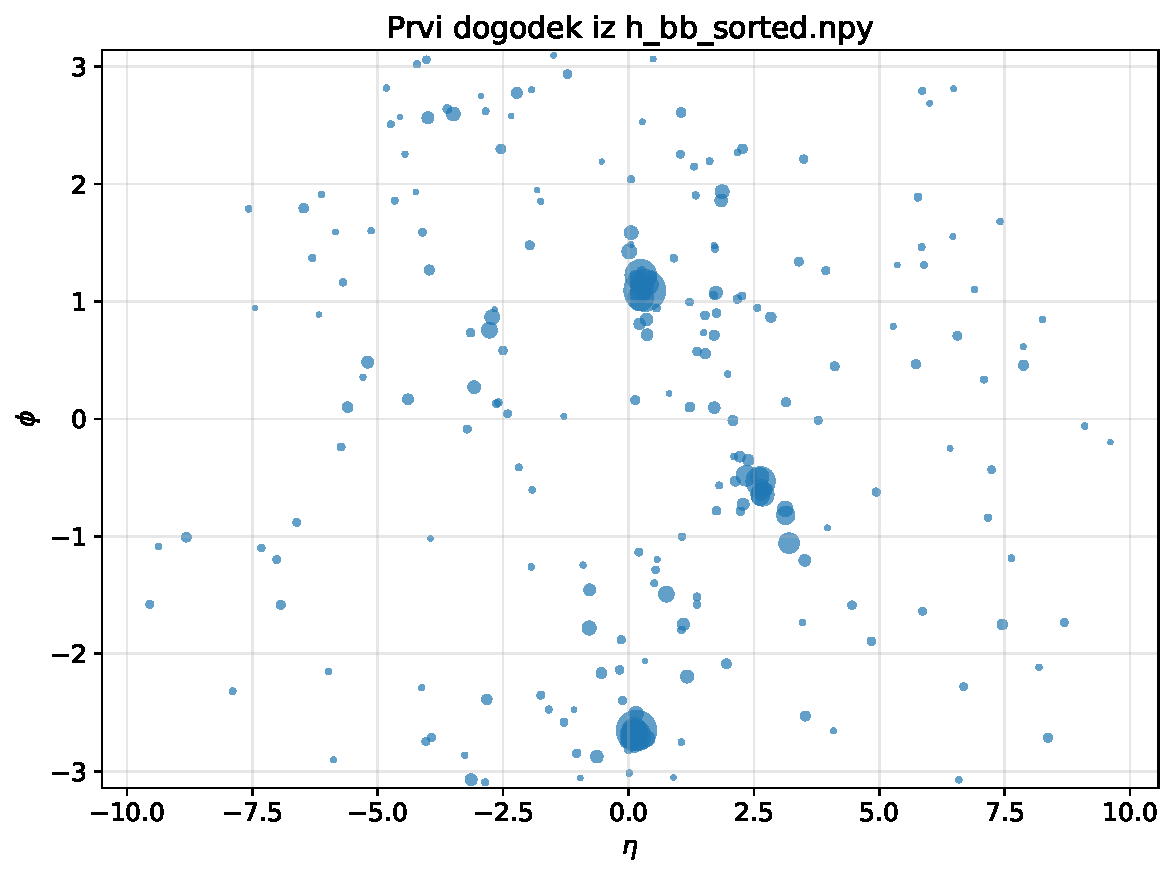
\includegraphics[width=0.75\textwidth]{imgs/event_display.pdf}
    \caption{Prikaz dogodka v detektorju. Na sliki so prikazani delci, ki jih je zaznal detektor. Vsak delec je predstavljen z eno točko, ki je določena s svojo pseudorapidnostjo $\eta$ in azimutalnim kotom $\phi$. Velikost točke predstavlja tranzverzalno gibalno količino $p_T$ delca.}
    \label{fig:event_display}
\end{figure}


Pri algoritmu K-means je potrebno določiti število gruč $K$. To lahko storimo tako, da pognamo algoritem za različna števila gruč in izračunamo povprečno razdaljo točk do najbližjega centroida. Rezultati so prikazani na sliki \ref{fig:kmeans_results}. Na sliki je prikazana povprečna razdalja (cenilka) točk do najbližjega centroida v odvisnosti od števila gruč $K$ ter rekonstruirana masa Higgsovega bozona v odvisnosti od števila gruč $K$. Masa je izračunana kot $m_h = \sqrt{(E_1 + E_2)^2 - (\mathbf{p}_1 + \mathbf{p}_2)^2}$, kjer $E_{1,2} \approx |\mathbf{p}_{1,2}|$ predstavljata energijo obeh curkov, ter $\mathbf{p}_{1,2}$ predstavljata njihovo gibalno količino. S črtkano modro črtico je prikazana znana masa Higgsovega bozona.

Vidimo, da cenilka pada z naraščanjem števila gruč, kar je pričakovano, saj večje število gruč pomeni manjše razdalje do najbližjega centroida. Rekonstruirana masa Higgsovega bozona pa se stabilizira pri $K=14$, kar pomeni, da je to optimalno število gruč za ta dogodek.


\begin{figure}[h!]
    \centering
    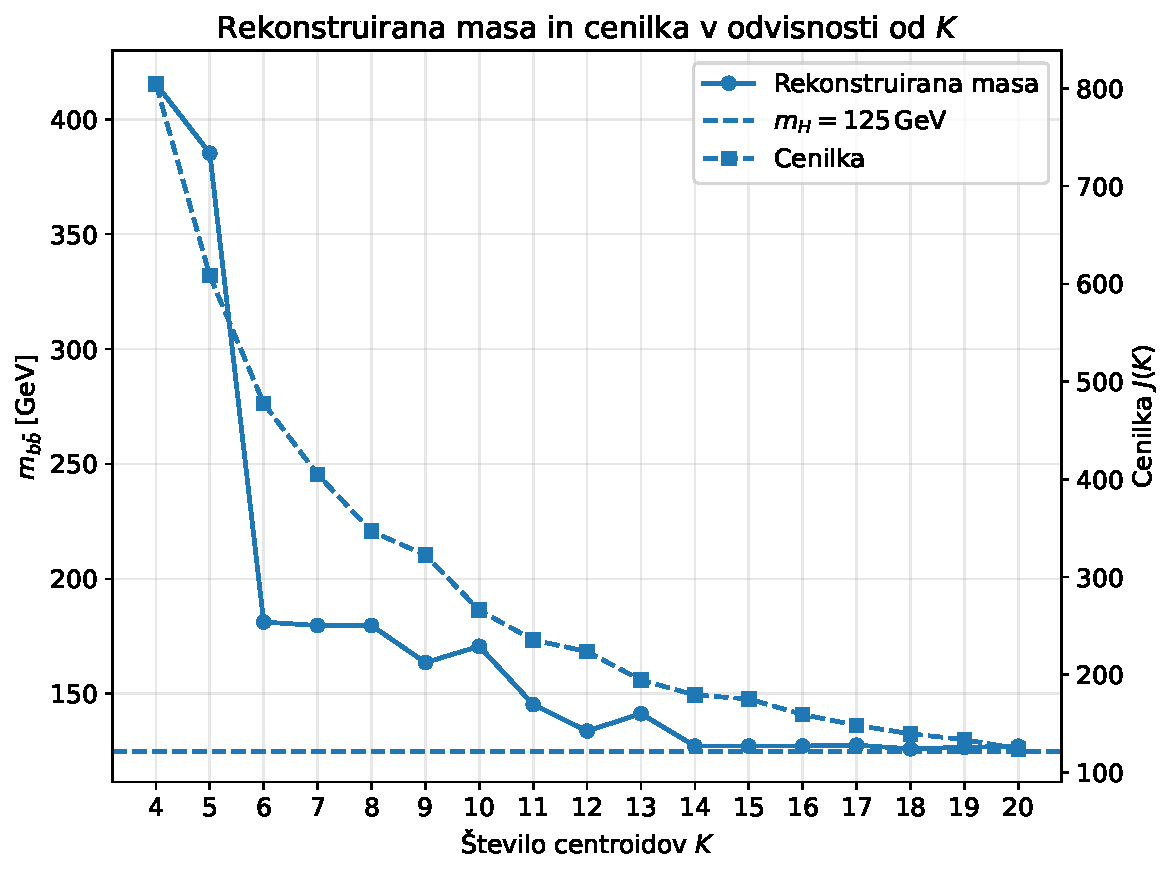
\includegraphics[width=0.75\textwidth]{imgs/kmeans_results.pdf}
    \caption{Povprečna razdalja (cenilka) točk do najbližjega centroida v odvisnosti od števila gruč $K$ ter rekonstruirana masa Higgsovega bozona v odvisnosti od števila gruč $K$.}
    \label{fig:kmeans_results}
\end{figure}


Na sliki \ref{fig:kmeans_results_2} sta prikazana centroida dveh gruč z največjo gibalno količino $p_T$, ki ju je našel K-means algoritem za $K=14$. Delci, ki pripadajo glavnim centroidom, so prikazani z oranžno ter zeleno barvo. Vidimo, da se centroida nahajata pri $\phi \approx -2.6$ ter $\phi \approx 1.1$, kar je v skladu z našimi pričakovanji.


\begin{figure}[h!]
    \centering
    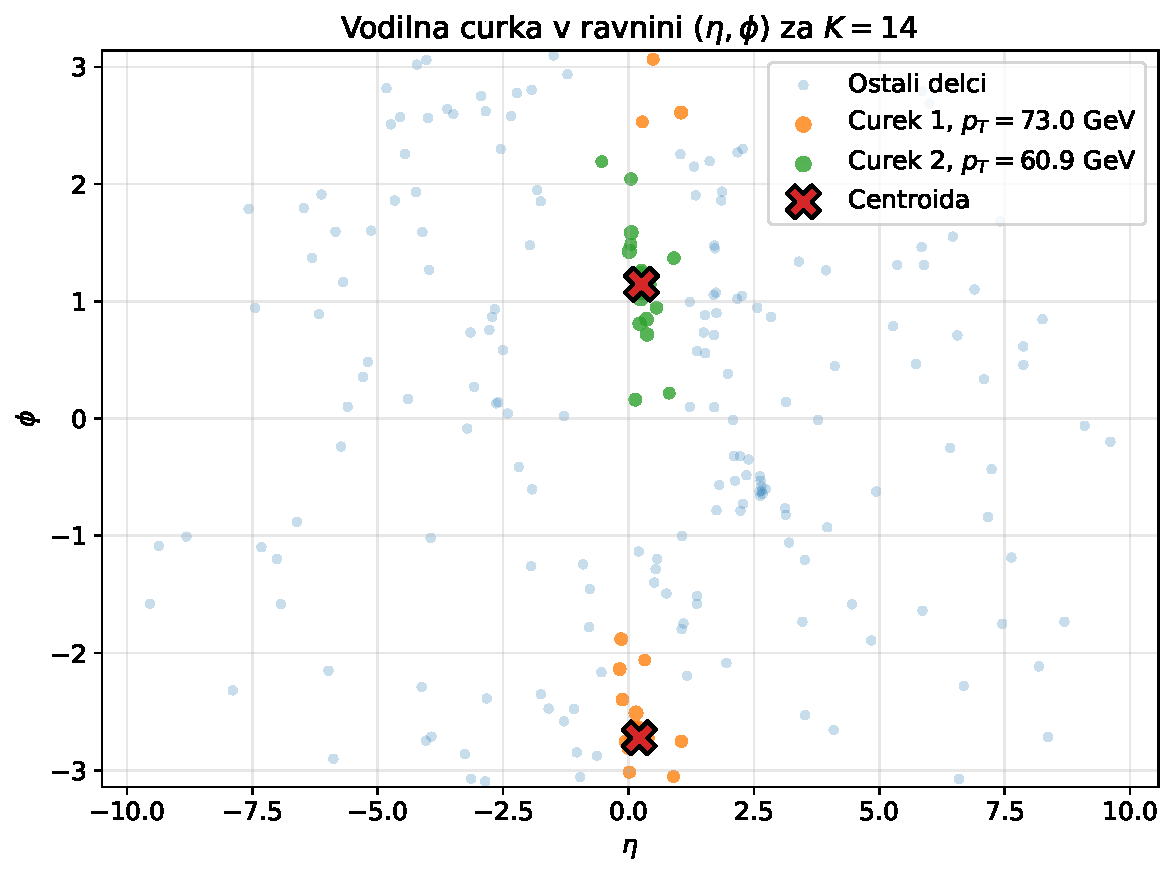
\includegraphics[width=0.75\textwidth]{imgs/kmeans_results_2.pdf}
    \caption{Centroida dveh gruč z največjo gibalno količino $p_T$, ki ju je našel K-means algoritem za $K=14$.}
    \label{fig:kmeans_results_2}
\end{figure}


\subsection{Infrardeča varnost}


\begin{figure}[h!]
    \centering
    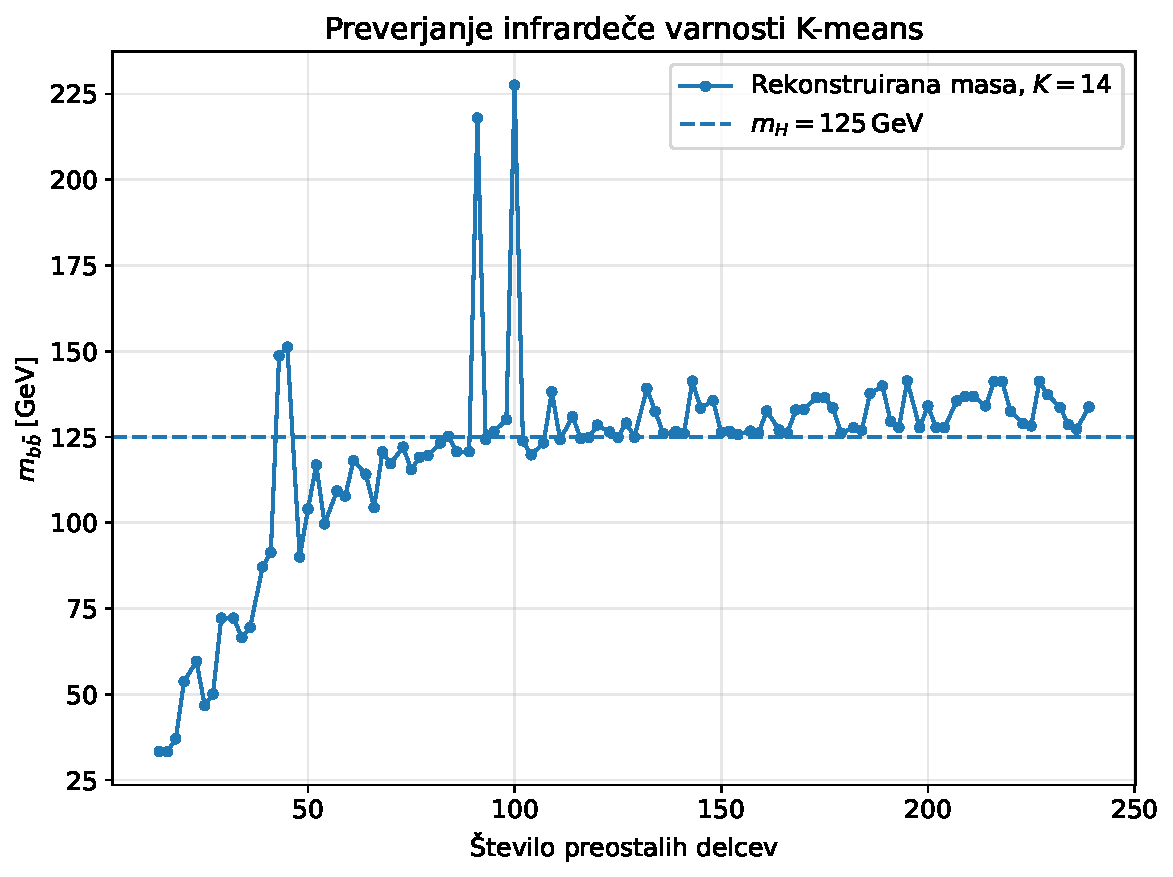
\includegraphics[width=0.75\textwidth]{imgs/kmeans_infrardeca.pdf}
    \caption{Centroida dveh gruč z največjo gibalno količino $p_T$, ki ju je našel K-means algoritem za $K=14$.}
    \label{fig:kmeans_infrardeca}
\end{figure}


Rezultati gručenja ne smejo biti občutljivi na odvzemanje delcev z nizko gibalno količino $p_T$, saj ti delci ne pripadajo glavnim curkom. To lahko preverimo tako, da odstranjujemo delce z majhno gibalno količino $p_T$ in ponovno pognemo K-means algoritem ter izračunamo maso Higgsovega bozona. Rezultati so prikazani na sliki \ref{fig:kmeans_infrardeca}. Vidimo, da se masa Higgsovega bozona ne spreminja dokler ne ostane cca 80 delcev, kar pomeni, da je K-means algoritem odporen na odvzemanje delcev z nizko gibalno količino $p_T$.

\section{Algoritem hierarhičnega gručenja}

Za izbiro parametra $R$ sem pognal algoritem za različne vrednosti $R$ in izračunal maso Higgsovega bozona. Rezultati so prikazani na sliki \ref{fig:hierarchical_clustering}. Vidimo, da se masa Higgsovega bozona za vse vrednosti $k$ stabilizira pri $R \approx 0.6$, kar pomeni, da je to optimalna vrednost parametra $R$ za ta dogodek. To sem se odločil tudi s pomočjo vizualnega testa.


\begin{figure}[h!]
    \centering
    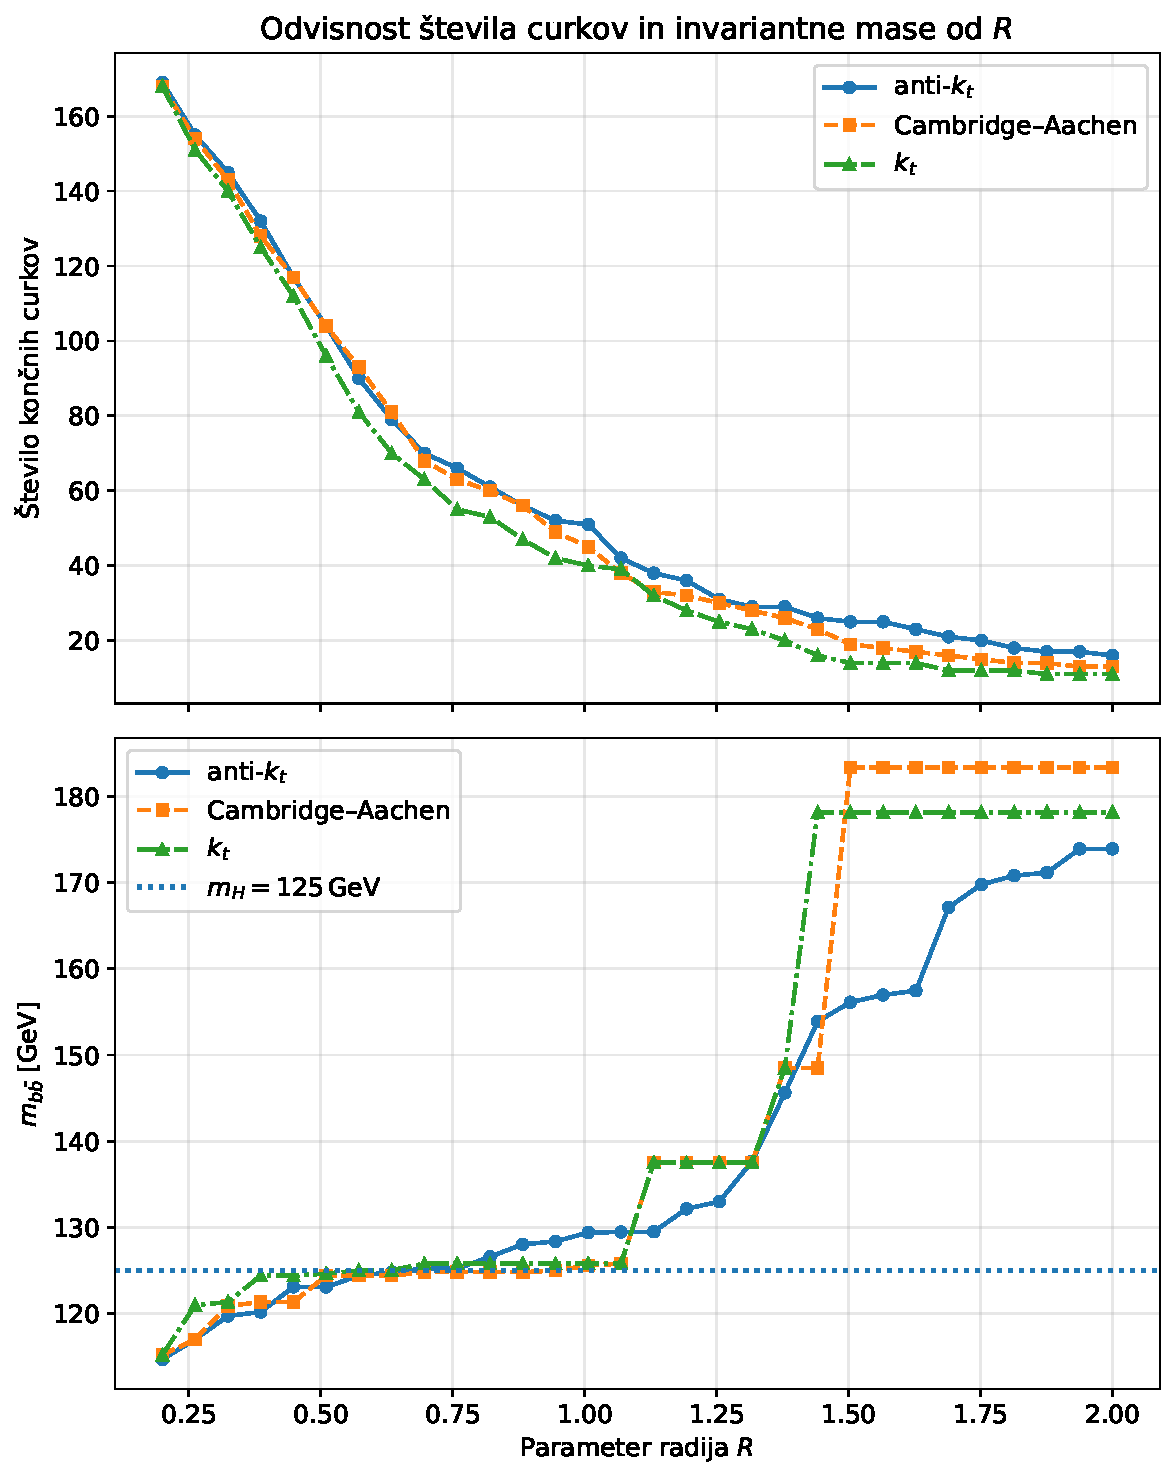
\includegraphics[width=0.8\textwidth]{imgs/hierarchical_clustering.pdf}
    \caption{Število gruč v odvisnosti od parametra $R$ ter Rekonstruirana masa Higgsovega bozona v odvisnosti od parametra $R$.}
    \label{fig:hierarchical_clustering}
\end{figure}


Na zgornjem grafu je prikazano število gruč v odvisnosti od parametra $R$. Vidimo, da se število gruč zmanjšuje z naraščanjem parametra $R$, kar je pričakovano, saj večji parameter $R$ pomeni večjo verjetnost, da se bodo protocurki združili v eno gruče.


\subsection{Infrardeča varnost ter čas izvajanja}

Tudi za hierarhično gručenje lahko preverimo preveril infrardečo varnost. Rezultati so prikazani na sliki \ref{fig:hierarhicno_comparison}. Prikazana sta implementirani algoritem ter algoritem iz knjižnice \texttt{pyjet}.

Vidimo, da je ta krivulja precej bolj gladka kot pri K-means algoritmu. Pri cca 60 preostalih delcih se masa Higgsovega bozona spremeni za približno 7 GeV (5\%), kar je še vedno sprejemljivo. To pomeni, da je hierarhični algoritem odporen na odvzemanje delcev z nizko gibalno količino $p_T$.


\begin{figure}[h!]
    \centering
    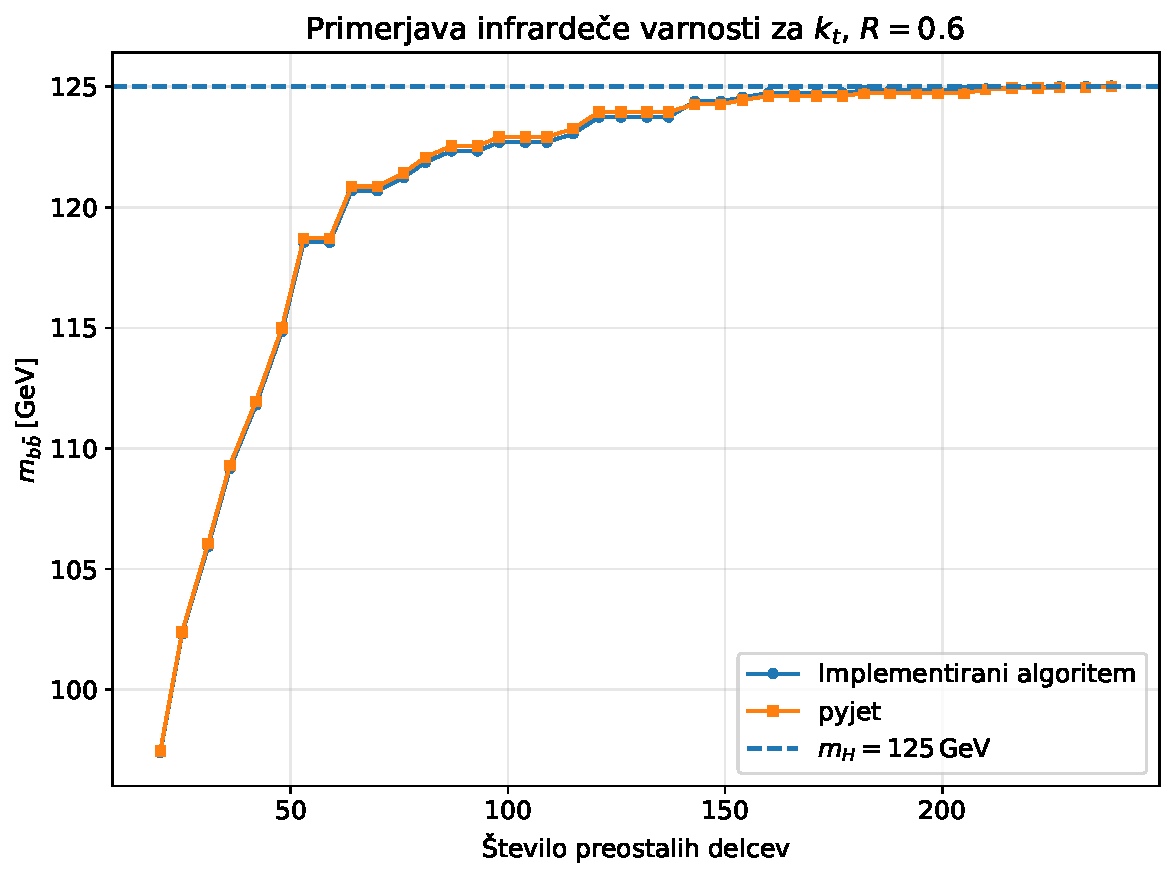
\includegraphics[width=0.8\textwidth]{imgs/hierarhicno_comparison.pdf}
    \caption{Infrardeča varnost hierarhičnega gručenja. Prikazana sta implementirani algoritem ter algoritem iz knjižnice \texttt{pyjet}.}
    \label{fig:hierarhicno_comparison}
\end{figure}


Merimo lahko tudi čas izvajanja implementiranega algoritma hierarhičnega gručenja ter algoritma iz knjižnice \texttt{pyjet}. Rezultati so prikazani na sliki \ref{fig:time_complexity}. Vidimo, da je čas izvajanja implementiranega algoritma večji kot čas izvajanja algoritma iz knjižnice \texttt{pyjet}. To je pričakovano, saj je implementirani algoritem bolj preprost in ne uporablja optimizacij, ki jih uporablja knjižnica \texttt{pyjet}.


\begin{figure}[H]
    \centering
    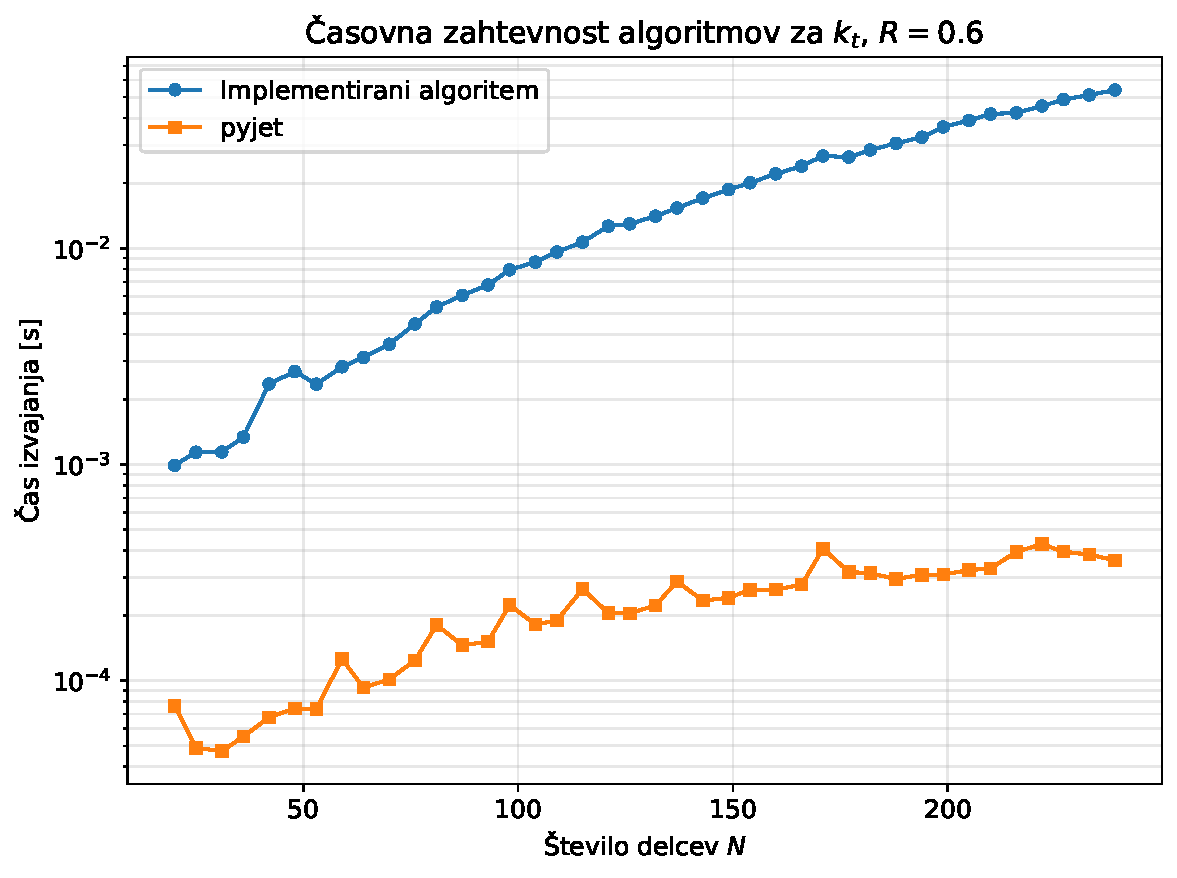
\includegraphics[width=0.8\textwidth]{imgs/time_complexity.pdf}
    \caption{Čas izvajanja hierarhičnega gručenja v odvisnosti od števila delcev $N$.}
    \label{fig:time_complexity}
\end{figure}


\section{Rekonstrukcija mase Higgsovega bozona}

Sedaj smo pripravljeni, da rekunstruiramo maso Higgsovega bozona iz vseh dogodkov. Za vsak dogodek bomo uporabili hierarhični algoritem gručenja iz knjižnice \texttt{pyjet} z parametrom $R=0.6$. Za vsak dogodek bomo izluščili dva curka z največjo gibalno količino $p_T$ ter izračunali maso Higgsovega bozona. Histogram vrednosti izračunanih mas je prikazan na sliki \ref{fig:reconstructed_masses}. Vidimo, da je histogram skoncentriran okoli 125 GeV, kar je v skladu z znano maso Higgsovega bozona.


\begin{figure}[h!]
    \centering
    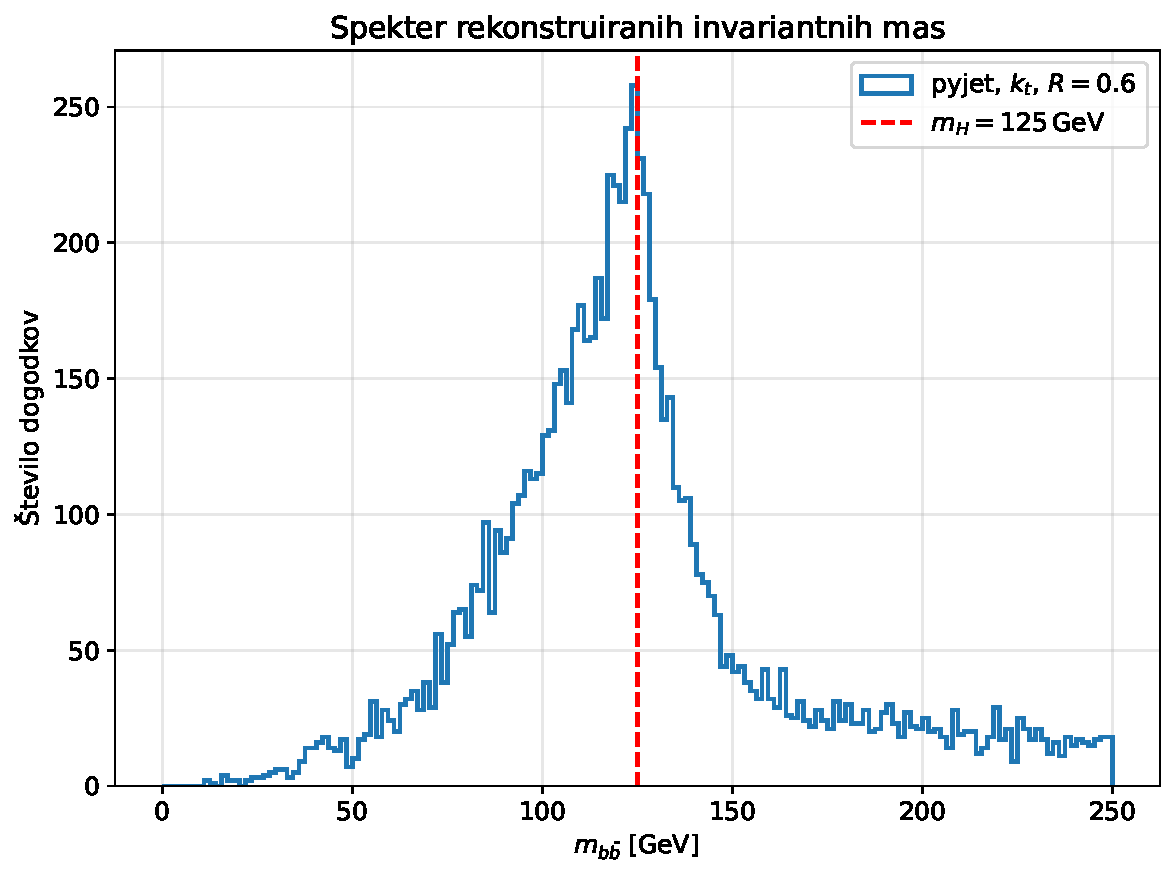
\includegraphics[width=0.8\textwidth]{imgs/reconstructed_masses.pdf}
    \caption{Histogram izračunanih mas Higgsovega bozona iz vseh dogodkov.}
    \label{fig:reconstructed_masses}
\end{figure}


Na ta histogram lahko priležemo funkcijo Crystal Ball, ki smo jo spoznali v prvi nalogi. Ta je kombinacija Gaussovega jedra ter debelejših repov in je definirana kot


\begin{equation}
    \begin{cases}
        CB =
        \dfrac{e^{-(m-m_{CB})^2/(2\sigma_{CB}^2)}}{\sqrt{2\pi}\sigma_{CB}}, & -\alpha_L < \dfrac{m-m_{CB}}{\sigma_{CB}} < \alpha_R, \\
        \left(\dfrac{n_L}{|\alpha_L|}\right)^{n_L} e^{-\alpha_L^2/2}
        \left(\dfrac{n_L}{|\alpha_L|} - |\alpha_L| - \dfrac{m-m_{CB}}{\sigma_{CB}}\right)^{-n_L}, & \dfrac{m-m_{CB}}{\sigma_{CB}} \le -\alpha_L, \\
        \left(\dfrac{n_R}{\alpha_R}\right)^{n_R} e^{-\alpha_R^2/2}
        \left(\dfrac{n_R}{\alpha_R} - \alpha_R + \dfrac{m-m_{CB}}{\sigma_{CB}}\right)^{-n_R}, & \dfrac{m-m_{CB}}{\sigma_{CB}} \ge \alpha_R,
    \end{cases}
\end{equation}
kjer so $m_{CB}, \sigma_{CB}, \alpha_L, n_L, \alpha_R, n_R$ prosti parametri.


Rezultati prileganja so prikazani na sliki \ref{fig:double_crystal_ball_fit}. Vidimo, da je prilegana funkcija dobro prilagojena histogramu, kar pomeni, da je funkcija Crystal Ball primerna za opisovanje porazdelitve mas Higgsovega bozona. Izračunana masa Higgsovega bozona je $m_{CB} = 124.5 \pm 1$ GeV, kar je v skladu z znano maso Higgsovega bozona.


\begin{figure}[H]
    \centering
    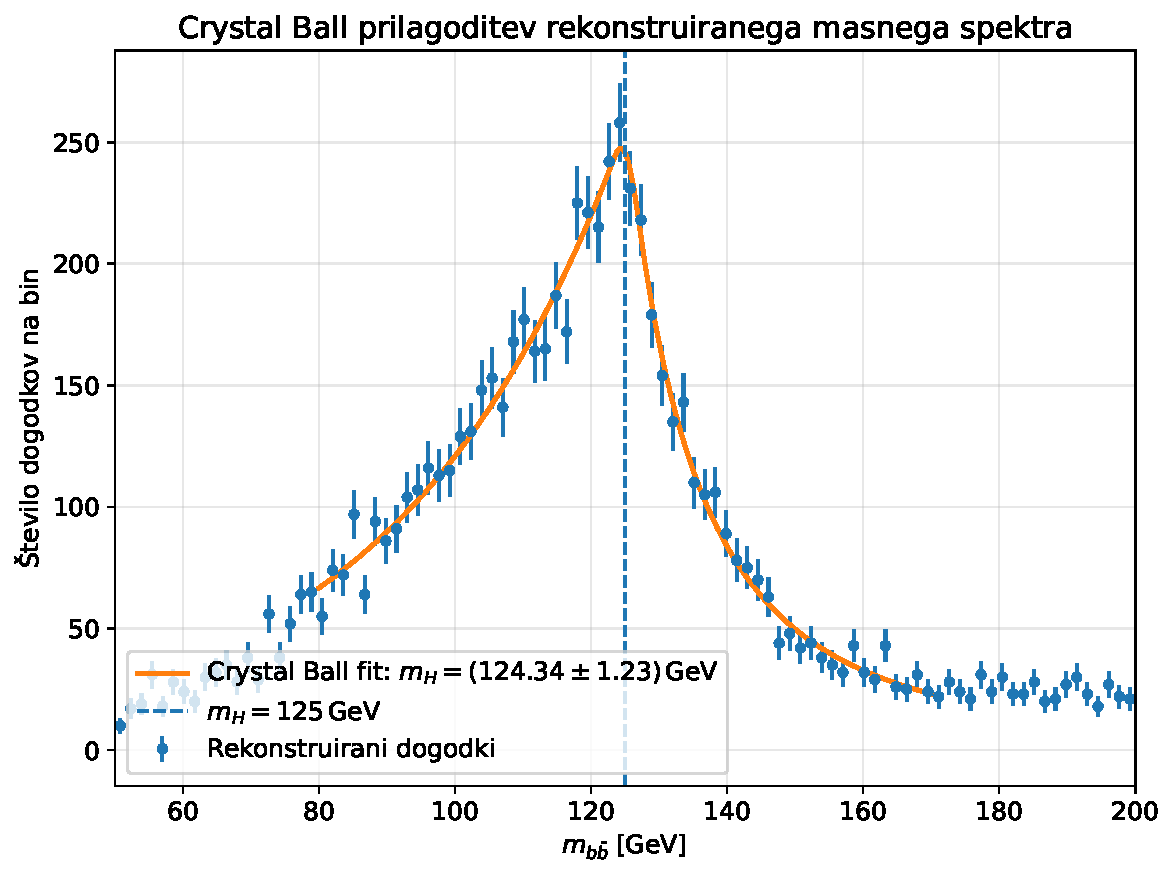
\includegraphics[width=0.8\textwidth]{imgs/double_crystal_ball_fit.pdf}
    \caption{Histogram izračunanih mas Higgsovega bozona iz vseh dogodkov ter prilegana funkcija Crystal Ball.}
    \label{fig:double_crystal_ball_fit}
\end{figure}


\section{Zaključek}

V tem poročilu smo uporabili algoritme gručenja za analizo podatkov iz trkov delcev. Uporabili smo K-means ter hierarhično gručenje, da smo iz podatkov izluščili dva hadronska curka z največjo gibalno količino $p_T$. Iz teh dveh curkov smo lahko izračunali maso Higgsovega bozona.

Rezultati so pokazali, da sta oba algoritma primerena za ta problem, saj sta našla dva centra skupin, ki sta bila v skladu z našimi pričakovanji. Prav tako sta bila oba algoritma odporna na odvzemanje delcev z nizko gibalno količino $p_T$, kar pomeni, da sta infrardečno varna.

Z algoritmom hierarhičnega gručenja iz knjižnice \texttt{pyjet} smo iz vseh dogodkov izluščili dva curka z največjo gibalno količino $p_T$ ter izračunali maso Higgsovega bozona. Histogram izračunanih mas je bil skoncentriran okoli 125 GeV, kar je v skladu z znano maso Higgsovega bozona. Prileganje funkcije Crystal Ball je pokazalo, da je ta funkcija primerna za opisovanje porazdelitve mas Higgsovega bozona, saj smo za rezultat dobili maso $m_{CB} = 124.5 \pm 1$ GeV, kar je v skladu z znano maso Higgsovega bozona.

\end{document}